\documentclass[conference]{IEEEtran}
\IEEEoverridecommandlockouts
% The preceding line is only needed to identify funding in the first footnote. If that is unneeded, please comment it out.
\usepackage{cite}
\usepackage{amsmath,amssymb,amsfonts}
\usepackage{algorithmic}
\usepackage{graphicx}
\usepackage{textcomp}
\usepackage{xcolor}
\usepackage{bm}
\usepackage{hyperref}
\hypersetup{
  colorlinks, linkcolor=red
}
\def\BibTeX{{\rm B\kern-.05em{\sc i\kern-.025em b}\kern-.08em
    T\kern-.1667em\lower.7ex\hbox{E}\kern-.125emX}}
\begin{document}

\title{Trajectory Optimization for an Inertial Cube \\
}

\author{\IEEEauthorblockN{Ethan Weber}
\IEEEauthorblockA{\textit{6.832 (Underactuated Robotics) Final Project} \\
\textit{Massachusetts Institute of Technology}\\
Cambridge, MA \\
ejweber@mit.edu}
}

\maketitle

\begin{abstract}
Inertially-actuated robots pose interesting problems for underactuated control. Here we present a trajectory opimization method to control a 2d cube with a torque-limited flywheel mounted inside. Inspired by earlier work done with the Cubli \cite{b2} and M-Blocks \cite{b3}, we use contact-implicit trajectory optimization to generate trajectories for the inerial cube. We use one actuator (the flywheel) to control the 8 states of the robot over time. Using Sparse Nonlinear OPTimizer (SNOPT) in Drake, the interial cube can be descriped as a floating body with contact implicit movements via linear complementarity contraints. This leads to elegant optimal trajectory control for the interial cube.
\end{abstract}

\begin{IEEEkeywords}
trajectory optimization, underactuated, inertia, contact-implicit
\end{IEEEkeywords}

\section{Introduction}
The inertial cube is particularly interesting both due to its extreme underactuation and its simplicity. After seeing the potential of M-Blocks \cite{b3}, it's clear that inertially-actuated cubes have potential to be used in a variety of applications. The posibilities of movements are great, as seen in this video \url{https://www.youtube.com/watch?v=Nns0qzd8Noo}. The cubli also presents very nice control in stabilization to resist movement \url{https://www.youtube.com/watch?v=n_6p-1J551Y}. By combining prior work with ideas from optimal control and trajectory optimization, the inertial cube has potential for much more complex behavior. With elegant algorithms, we may be able to help robots explore extraterrestrial space \cite{b6} or create configurable robots like the nanobots in the movie \textit{Big Hero 6}. We are interested in applying our best underactuated control algorithms to the system.

\section{Defining the Model}

In this section, we describe the interial cube in floating-body coordinates with a few simplifying assumptions. The dynamics work out nicely when described in this way. We can then proceed to optimize over the state trajectory, input torque, and external contact forces over time.

\subsection{State Space Explanation}

Fig.~\ref{fig:cube} is a diagram depicting the states of the cube. The cube is defined in floating-coordinates, meaning there is no notion of the ground in the state description. However, there are a 4 contact vectors, 1 for each corner. These are described in the figure.

\begin{figure}[htbp]
\centerline{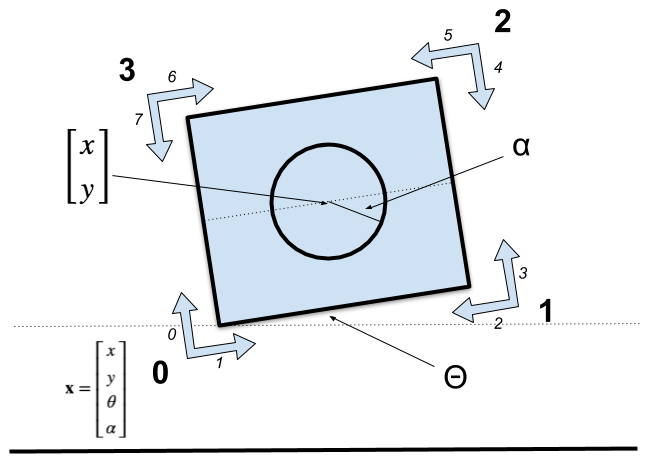
\includegraphics[width=9cm,keepaspectratio]{media/cube_states.png}}
\caption{The states of the floating inertial cube. The derivates of these states are also included in the total state vector $\textbf{x}$ but are not shown here for convenience.}
\label{fig:cube}
\end{figure}

Following from the cube diagram, the full states can be described in the following way. \\

\begin{align}
  \textbf{x} =
    \begin{bmatrix}
         x \\
         y \\
         \theta \\
         \alpha \\
         \dot x \\
         \dot y \\
         \dot \theta \\
         \dot \alpha
    \end{bmatrix} &&
  \bm{\dot x} =
    \begin{bmatrix}
         \dot x \\
         \dot y \\
         \dot \theta \\
         \dot \alpha \\
         \ddot x \\
         \ddot y \\
         \ddot \theta \\
         \ddot \alpha
    \end{bmatrix}
\end{align}

These state vector $\textbf{x}$ includes both the positions, angles, and their velocities. This is standard state-space notation. Following from Fig.~\ref{fig:cube}, the dynamics are the following. These dynamics are informed by prior work done at Chalmers University of Technology \cite{b4} but modified for this state-space description and free-body coordinates.

\begin{align}
\ddot x &= (f_{1}-f_{2}+f_{6}-f_{5})\cos{\theta} - (f_{0}+f_{3}-f_{4}-f_{7})\sin{\theta} \\
\ddot y &= (f_{1}-f_{2}+f_{6}-f_{5})\sin{\theta} + (f_{0}+f_{3}-f_{4}-f_{7})\cos{\theta}-g \\
\ddot \theta &= \frac{-u + b_{w}\dot\alpha - b_{c}\dot\theta}{I_c} + \frac{1}{2}(\sum_{\set{n\in{1,3,5,7}}} f_{n} - \sum_{\set{n\in{0,2,4,6}}} f_{n}) \\
\ddot \alpha &= \frac{u(I_{c}+I{w}) + b_{c}I_{w}\dot\theta - b_{w}\frac{I_{c}+I_{w}}{2}\dot\alpha}{I_{w}I_{c}}
\end{align}

Here we explain the notation used in the dynamics and the few simple assumptions made. \\
\begin{itemize}
\item $f_{n}$ is the force acting on the corner based on Fig.~\ref{fig:cube}.
\item $u$ is the torque on the interial wheel.
\item The cube is unit sized, meaning its dimensions are 1 for each edge length.
\item 
\end{itemize}




\section{Optimization Formulation}
In this section, we explain the necessary nonlinear program formulation to solve for a cube trajectory through space. We'll start by explaining this in the context of a simple swing up of the cube. This motion involves contact with the ground, which is why we are choosing do use contact-implicit trajectory optimization to avoid dealing with many modes of the system \cite{b1}.

\subsection{The Simple Swing-Up}
The swing-up is performed by getting the cube to stand on exactly one corner in a stable position. By using the contact-implicit trajectory optimization, this is possible. The computed trajectory values are showing in Fig. \ref{fig:swing_states}, \ref{fig:swing_input}, and \ref{fig:swing_ground}. This computed result is formated without a cost function. Rather, we are looking for a solution the satisfied all of our constraints.

\begin{figure}[htbp]
\centerline{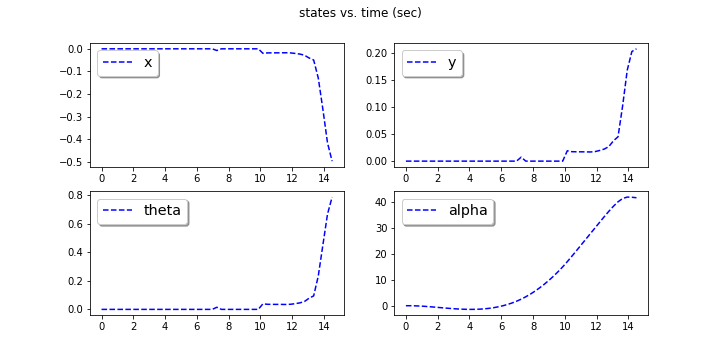
\includegraphics[width=9cm,keepaspectratio]{media/swing_up/swing_up_states.png}}
\caption{Swing up trajectory states.}
\label{fig:swing_states}
\centerline{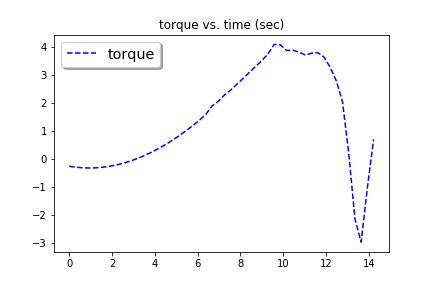
\includegraphics[width=9cm,keepaspectratio]{media/swing_up/swing_up_torque.png}}
\caption{Swing up trajectory torque input.}
\label{fig:swing_input}
\centerline{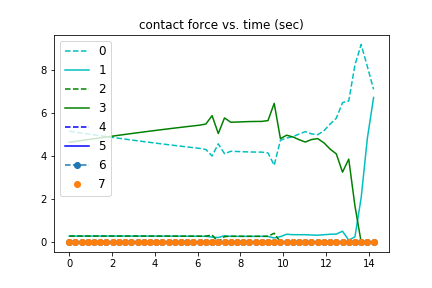
\includegraphics[width=9cm,keepaspectratio]{media/swing_up/swing_up_ground_forces.png}}
\caption{Swing up trajectory ground forces.}
\label{fig:swing_ground}
\end{figure}

Explain that LQR could be used to control after achieving swing up.

\subsection{Experiments in Higher Dimensional State Space}
Explain how 3D seemed to help in some cases even though some states don't enter dynamics.

\subsection{Stable Walking Motion}

Explain how to achieve stable walking motion.

\section*{Results}

Explanation of results section. This should include more diagrams.

\section*{Future Work}

Future work section.

\begin{thebibliography}{00}
\bibitem{b1} M. Posa, C. Cantu, and R. Tedrake. ``A Direct Method for Trajectory Optimization of Rigid Bodies Through Contact,'' in The International Journal of Robotics Research, 2014 \url{http://groups.csail.mit.edu/robotics-center/public_papers/Posa13.pdf}
\bibitem{b2} M. Gajamohan, M. Merz, I. Thommen, and R. D'Andrea. ``The Cubli: A Cube that can Jump Up and Balance,'' in IEEE/RSJ International Conference on
Intelligent Robots and Systems, 2012 \url{https://www.ethz.ch/content/dam/ethz/special-interest/mavt/dynamic-systems-n-control/idsc-dam/Research_DAndrea/Cubli/Cubli_IROS2012.pdf}
\bibitem{b3} J. Romaniskin, K. Gilpin, and D. Rus. ``M-Blocks: Momentum-driven, Magnetic Modular Robots,'' in Proc. IROS, IEEE/RSJ, 2013
\url{http://citeseerx.ist.psu.edu/viewdoc/download?doi=10.1.1.824.7275&rep=rep1&type=pdf}
\bibitem{b4} E. Bjerke, B. Pehrsson. ``Development of a Nonlinear Mechatronic Cube,'' Chalmers University of Technology, 2016
\url{http://publications.lib.chalmers.se/records/fulltext/233543/233543.pdf}
\bibitem{b5} Y. Dauphin, R. Pascanu, C. Gulcehre, K. Cho, S. Ganguli, and Y. Bengio. ``Identifying and attacking the saddle point problem in high-dimensional non-convex optimization,'' in Proceedings of the 27th International Conference on Neural Information Processing Systems - Volume 2, 2014
\url{https://ganguli-gang.stanford.edu/pdf/14.SaddlePoint.NIPS.pdf}
\bibitem{b6} B. Hockman and M. Pavone. ``Stochastic Motion Planning for Hopping Rovers on Small Solar System Bodies,'' in Int. Symp. on Robotics Research, 2017
\url{https://asl.stanford.edu/wp-content/papercite-data/pdf/Hockman.Pavone.ISRR17.pdf}
\end{thebibliography}


\vspace{12pt}

\end{document}
